\documentclass[11pt,a4paper]{article}

\usepackage{fontspec}
\usepackage{microtype}
\usepackage[margin=2.5cm]{geometry}
\usepackage{amsmath,amssymb}
\usepackage{booktabs,tabularx,array}
\usepackage{enumitem}
\usepackage{caption}
\usepackage{tikz}
\usetikzlibrary{positioning,arrows.meta,calc}
\usepackage[hidelinks]{hyperref}

\captionsetup{font=small,labelfont=bf}
\setlist{itemsep=2pt,topsep=4pt}
\newcolumntype{L}{>{\raggedright\arraybackslash}X}
\newcommand{\code}[1]{\texttt{#1}}
\newcommand{\repourl}{https://github.com/BierschneiderEmanuel/pWaveDetection}
\newcommand{\repofile}[2]{\href{\repourl/blob/main/#2}{\code{#1}}}
\newcommand{\repodir}[2]{\href{\repourl/tree/main/#2}{\code{#1}}}
\newcommand{\ms}{\,\mathrm{ms}}
\renewcommand{\arraystretch}{1.15}
\setlength{\emergencystretch}{2em}

\title{Conventional P-Wave Detection in a Single-Lead 128\,Hz ECG:\\
\large A Rule-Based Detector Paired with a Learned Candidate Scorer, Assessed Patient-Wise Across Four Annotated Databases}
\author{Emanuel Bierschneider}
\date{October 2026}

\begin{document}
\maketitle

\begin{abstract}
\noindent
A P-wave peak detector that relies on no neural networks attains a macro-averaged $F_1$ of 92.0\,\% when scored on held-out test patients. The macro average is computed across four annotated ECG databases.

The detector operates on a single ECG lead resampled to 128\,Hz. R peaks are located with the Elgendi (2013) algorithm, and a search is then carried out up to 300\,ms to the left of every R peak, terminating just before an estimated QRS onset. Within that window, band-limited candidate peaks are ranked by prominence, by a latency prior derived from a lead-level P template, and by shape correlation against that template. A candidate is only reported once it exceeds a robust noise floor built from high-frequency MAD and from low-frequency activity within the window.

Two detectors build on this shared front end. The rule detector admits candidates through a cascade of rules: a relative amplitude gate bounded by an absolute cap; an ectopy gate grounded in QRS shape correlation; a second pass that enforces beat-to-beat PR-latency consistency; and sub-sample parabolic interpolation. The learned detector substitutes the acceptance rules with a logistic-regression scorer trained over 22 hand-crafted candidate features.

The four databases were converted into a single JSON format and partitioned into train, validation and test sets of 60/20/20\,\% by source patient: BUT PDB, PhysioNet PWAVE, LUDB and QTDB. All fitting was performed on the training split. The validation split served selection only, and the test split was scored a single time.

\medskip
\begin{center}
\begin{tabular}{lccc}
\toprule
Detector & Train $F_1$ & Validation $F_1$ & Test $F_1$ \\
\midrule
Rule detector & 87.59\,\% & 85.51\,\% & 90.28\,\% \\
Learned detector (rules + logistic regression) & 89.03\,\% & 87.68\,\% & 92.02\,\% \\
\bottomrule
\end{tabular}
\end{center}
\medskip

Every figure is a macro $F_1$ measured at a $\pm50$\,ms matching tolerance. For the learned detector, per-database test $F_1$ spans from 89.3\,\% (QTDB) to 95.4\,\% (PWAVE). Gradient-boosted trees fitted the training set more closely yet generalised more poorly, and were therefore dropped on validation. The 95\,\% patient-bootstrap interval on the learned detector's test macro $F_1$ is 88.7--94.5\,\%, and its advantage over the rule detector is $+1.7$ points $[+0.2, +4.0]$. In atrial fibrillation, the learned detector reports a spurious P wave in 10.4 of every 100 test beats, versus 2.0 outside AF. Omitting the PR-consistency rule, the rule detector reports 23.4.
\end{abstract}

% ------------------------------------------------------------------
\section{Introduction}

The P wave is the electrical signature of atrial depolarisation, and detecting it reliably is what allows a rhythm to be classified as sinus. Whether it is present, when it occurs, and how regular it is are what separate sinus rhythm from atrial fibrillation (AF) and from junctional and ventricular rhythms, and they are also what the PR interval is derived from. Three factors make detection difficult:
\begin{itemize}
\item P amplitude frequently lies between 0.05 and 0.25\,mV, the same order of magnitude as muscle noise and baseline wander.
\item Polarity is lead-dependent.
\item At fast rates the P wave can fuse with the preceding T wave.
\end{itemize}
Long-term and wearable recordings add further difficulty. Such recordings frequently use a single lead at a low sampling rate; here the rate is 128\,Hz.

Classical methods rely on wavelet transforms, phasor transforms, template matching, or Bayesian models, applied after the QRS complex has been located. More recent work has turned to deep convolutional networks, but these demand large labelled corpora, are difficult to interpret, and are costly to run on embedded hardware. This work intentionally sets aside neural networks in all their forms, including CNNs and ResNets. It draws only on signal processing and compact classical models such as logistic regression and decision-tree ensembles.

\paragraph{Design constraints.}
\begin{enumerate}
\item R peaks are supplied by the Elgendi (2013) QRS detector.
\item P waves are searched for only within the 300\,ms preceding each R peak.
\item Every detection must exceed an explicit, per-beat noise floor.
\item The detector operates on single leads resampled to 128\,Hz.
\item Performance is reported patient-wise on data that played no part in development.
\end{enumerate}

\paragraph{Contributions.}
\begin{enumerate}
\item Four public databases carrying P-wave peak annotations were converted into a single JSON format and resampled to 128\,Hz. The format also adds rhythm (AF) labels.
\item A transparent rule-based P detector whose rules are each aimed at a particular failure mode: LBBB, small chest-lead P waves, ectopic beats, and AF.
\item A learned candidate scorer that works from 22 interpretable features and logistic regression, while retaining the rule-based front end.
\item A leak-free evaluation protocol. It splits by patient group across databases using a hash, so that records belonging to the same MIT-BIH patient, which appear in three of the databases, never end up in two splits. Tuning, model selection and testing are kept strictly separate.
\end{enumerate}

\subsection{Related work}

No published detector is an exact match for this one, yet most of its components are well established. Classical P detectors share a single structure: detect the QRS, mark a search region before it, and select the P maximum inside that region. They differ in the transform applied to the signal and in the decision rules \cite{martinez2004,saclova2022}. The R-peak stage of this work is a direct implementation of Elgendi (2013) \cite{elgendi2013}.

\begin{table}[htbp]
\centering\small
\caption{Published P-wave detectors closest in spirit to this work, with the results as their authors reported them.}
\label{tab:related}
\begin{tabularx}{\textwidth}{>{\raggedright\arraybackslash}p{2.6cm}LL>{\raggedright\arraybackslash}p{3.3cm}}
\toprule
Method & Approach & Evaluation data & Reported P-wave result \\
\midrule
Martínez et al.\ 2004 \cite{martinez2004} & Dyadic wavelet transform. QRS located first, then P and T peaks, onsets and offsets within regions fixed by the QRS. & MITDB, QTDB, European ST-T, CSE & Mean delineation error within a single sampling interval. P sensitivity is not stated in the abstract. \\
Martínez, Alcaraz and Rieta 2010 \cite{martinez2010} & Phasor transform, which boosts small waves, used for single-lead delineation. & QTDB & Not extracted for this draft. \\
Elgendi, Meo and Abbott 2016 \cite{elgendi2016} & Two event-related moving averages, sized to the P duration (about 110\,ms) and to QTc (about 400\,ms), combined with a dynamic threshold. Relies on correct R detection. & 10 MITDB records, 21\,702 beats, 360\,Hz & Se 98.05\,\%, +P 97.11\,\% \\
Maršánová et al.\ 2019 \cite{marsanova2019} & Phasor transform plus PVC classification (no P search before a PVC) and rules for pathology, including a search for dissociated P in second-degree AV block. & 12 pathological MITDB records (the PWAVE annotations), physiological MITDB and QTDB records & Pathological Se 96.40\,\%, PP 85.84\,\%. Physiological Se 98.42\,\%, PP 99.98\,\%. \\
Šaclová et al.\ 2022 \cite{saclova2022} & Phasor transform, PVC detection from the QRS region, and adaptive demarcation of the search area. Rules for AF, PVC and other arrhythmias decide where to search, or whether to search at all. & MITDB P annotations, QTDB, BUT PDB & BUT PDB Se 93.07\,\%, PP 88.60\,\%. Pathological MITDB 96.40\,\% / 91.56\,\%. QTDB 99.23\,\% / 99.12\,\%. \\
\bottomrule
\end{tabularx}
\end{table}

Šaclová et al.\ \cite{saclova2022} also review a wider set of classical approaches: adaptive thresholding, wavelets, P templates with correlation, Kalman filtering, support vector machines, Prony's method, hidden Markov models and dynamic programming. Neural approaches fall outside the constraints of this work.

\paragraph{Shared with prior work.}
\begin{itemize}
\item A search region placed before the QRS. Here it spans 300\,ms, ends at the QRS onset, and is bounded by the previous beat.
\item Template correlation against an averaged P wave.
\item An R-relative amplitude threshold.
\item Skipping the P search before ectopic ventricular beats. The BUT group does this with a QRS-region PVC rule; here it is achieved with a QRS-shape correlation rule (Section~\ref{sec:gates}).
\end{itemize}

\paragraph{Not found in this form in the cited work.}
\begin{itemize}
\item The explicit per-candidate noise floor, which fuses high-frequency MAD with in-window low-frequency activity.
\item The two-pass beat-to-beat PR-latency consistency applied as a defence against AF.
\item The 22-feature logistic-regression candidate scorer.
\item The evaluation split by patient group across databases that share MIT-BIH patients.
\end{itemize}
This is not meant as a claim of novelty: PR-interval regularity is a long-standing clinical criterion, and the search was confined to the papers above.

\paragraph{Comparability.} Published figures cannot be compared directly with Section~\ref{sec:results}:
\begin{itemize}
\item The cited studies use the native sampling rates of their databases (128--500\,Hz) and, in most cases, only the first lead. This work uses 128\,Hz and every lead.
\item They evaluate whole databases. This work reports only on the held-out patients.
\item Their matching tolerances and scoring rules were not verified for this draft.
\end{itemize}
On BUT PDB, the closest benchmark, Šaclová et al.\ report Se 93.07\,\% and PP 88.60\,\% over all 50 records. This work reaches Se 89.6\,\% and PPV 91.3\,\% on its 12 test records, but only Se 75.6\,\% and PPV 80.6\,\% on its 7 validation records. The BUT PDB outcome therefore depends heavily on which records are scored.

% ------------------------------------------------------------------
\section{Data}

Four public databases with manual P-wave peak annotations were used, three of them sourced from PhysioNet \cite{physionet} (Table~\ref{tab:data}): 535 ECG files, 3070 lead signals, 78\,135 P labels and 26.4\,h of signal at 128\,Hz. Each lead is treated as an independent single-lead recording.

\begin{table}[htbp]
\centering\small
\caption{Databases after conversion: BUT PDB, the Brno University of Technology P-wave database; PWAVE, the PhysioNet P-wave annotations of MIT-BIH excerpts; LUDB, the Lobachevsky University database; QTDB, the PhysioNet QT Database (q1c annotations). Duration is measured at 128\,Hz.}
\label{tab:data}
\begin{tabular}{lrrrrrrr}
\toprule
Database & Files & Leads & P labels & QRS labels & Duration & Native rate & Leads with AF \\
\midrule
BUT PDB & 50 & 100 & 10\,858 & 15\,276 & 3.33\,h & 360 / 128\,Hz & 22 \\
PWAVE & 180 & 360 & 44\,092 & 49\,886 & 12.00\,h & 360\,Hz & 16 \\
LUDB & 200 & 2400 & 16\,797 & 21\,965 & 6.67\,h & 500\,Hz & 180 \\
QTDB & 105 & 210 & 6\,388 & 7\,056 & 4.44\,h & 250\,Hz & 2 \\
\bottomrule
\end{tabular}
\end{table}

\subsection{Sources}

\paragraph{BUT PDB \cite{butpdb}.} 50 two-minute, two-lead excerpts of long-term Holter recordings. They derive from the MIT-BIH Arrhythmia Database (records 1--38), the MIT-BIH Supraventricular Arrhythmia Database (records 39--43) and the Long-Term AF Database (records 44--50). Each lead carries P peaks (label \code{P-Wave}) and QRS positions taken from the source database. The excerpts are rich in pathology: AF, flutter, AV blocks, bundle-branch blocks, and ventricular and supraventricular ectopy.

\paragraph{PWAVE \cite{pwave}.} P-wave annotations for 12 MIT-BIH Arrhythmia records \cite{mitbih} (100, 101, 103, 106, 117, 119, 122, 207, 214, 222, 223, 231), each 30\,min long. QRS labels are taken from the MIT-BIH \code{.atr} beat files. Every record was divided into 15 two-minute files.

\paragraph{LUDB \cite{ludb}.} 200 ten-second, 12-lead recordings at 500\,Hz, with P, QRS and T delineation performed per lead by cardiologists. Each lead retains its own labels.

\paragraph{QTDB \cite{qtdb}.} 105 fifteen-minute two-lead recordings, of which a short section was annotated beat by beat (after the filtering below, a median of 30 and at most 85 normal beats per record) in the \code{q1c} files. Each file was cut to the annotated region $\pm2$\,s. Only q1c beats of type \code{N} serve as QRS references, so these files carry \code{label\_scope = beats}: only detections belonging to an annotated beat are scored.

\subsection{Common format}

Each database was converted into the BUT PDB JSON schema by \repofile{src/convert.py}{src/convert.py}. Every lead becomes one \code{recording} entry holding the signal at the native rate together with a copy resampled to 128\,Hz by polyphase filtering (\code{scipy.signal.resample\_poly}).
Labels are \code{\{name, coordinates: \{peak\}, decision: \{verdict\}\}}, with \code{P-Wave} marking P peaks and \code{QRS} marking R positions in seconds. Converted files additionally carry \code{annotated\_range \{start, end\}} and \code{label\_scope} (\code{all} or \code{beats}). All experiments use only the 128\,Hz signal.

\subsection{Rhythm labels}
\label{sec:rhythmlabels}

An \code{AF} label was appended to every file as intervals that tile the recording, each with verdict 1 for atrial fibrillation and 0 otherwise. Atrial flutter is counted as 0.
\begin{itemize}
\item \textbf{BUT PDB:} taken from the source rhythm annotations, from MIT-BIH for records 1--38 and from LTAFDB for records 44--50. Segment offsets were verified by exact beat matching against the source. SVDB records 39--43 have no rhythm annotations; their verdict 0 follows the BUT pathology table.
\item \textbf{PWAVE:} from the MIT-BIH rhythm annotations. AF occurs only in record 222.
\item \textbf{LUDB:} from the \code{Rhythms} column of \code{ludb.csv}. 15 records are in AF.
\item \textbf{QTDB:} the 15 MIT-BIH-derived records were aligned to the MIT-BIH beat files by beat matching. 88 records have no rhythm source and carry no AF label.
\end{itemize}
The AF labels are not used by the detector. They support stratified analysis: the consistency rule of Section~\ref{sec:consistency} is designed to suppress detections during AF.

% ------------------------------------------------------------------
\section{Methods}

The detector runs per lead. It locates R peaks, assembles a per-beat search window, extracts candidate peaks in a P band, and admits at most one P peak per beat (Figure~\ref{fig:pipeline}). In the rule detector a cascade of rule gates governs acceptance; in the learned detector a logistic-regression scorer makes that decision. Every frequency-selective filter is a zero-phase Butterworth filter, and smoothing is done with moving averages. The filters are applied via \code{filtfilt}. Signal amplitudes are expressed in the units of the source (mV). The final parameter values are given in Table~\ref{tab:params}.

\begin{figure}[htbp]
\centering
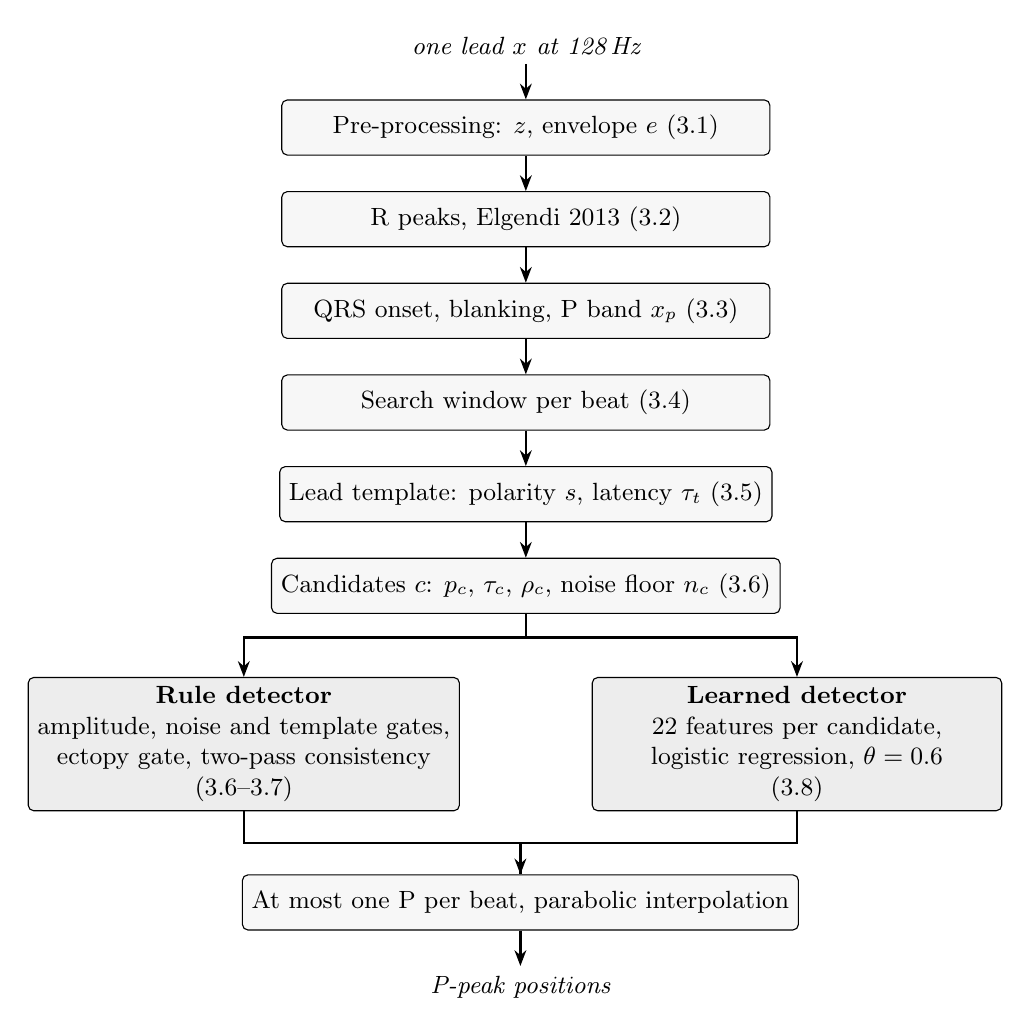
\begin{tikzpicture}[
  node distance=4.5mm and 6mm,
  box/.style={draw, rounded corners=2pt, align=center, font=\small, minimum width=6.2cm, minimum height=7mm, fill=gray!6},
  alt/.style={box, minimum width=5.2cm, fill=gray!14},
  io/.style={font=\small\itshape, align=center},
  arr/.style={-{Stealth[length=2mm]}, thick}]
\node[io]  (in)  {one lead $x$ at 128\,Hz};
\node[box, below=of in]  (pre) {Pre-processing: $z$, envelope $e$ (3.1)};
\node[box, below=of pre] (r)   {R peaks, Elgendi 2013 (3.2)};
\node[box, below=of r]   (on)  {QRS onset, blanking, P band $x_p$ (3.3)};
\node[box, below=of on]  (win) {Search window per beat (3.4)};
\node[box, below=of win] (tpl) {Lead template: polarity $s$, latency $\tau_t$ (3.5)};
\node[box, below=of tpl] (cand){Candidates $c$: $p_c$, $\tau_c$, $\rho_c$, noise floor $n_c$ (3.6)};
\node[alt, below left=8mm and -2.4cm of cand]  (rul) {\textbf{Rule detector}\\amplitude, noise and template gates,\\ectopy gate, two-pass consistency\\(3.6--3.7)};
\node[alt, below right=8mm and -2.4cm of cand] (lrn) {\textbf{Learned detector}\\22 features per candidate,\\logistic regression, $\theta = 0.6$\\(3.8)};
\coordinate (mid) at ($(rul.south)!0.5!(lrn.south)$);
\node[box, below=8mm of mid] (int) {At most one P per beat, parabolic interpolation};
\node[io, below=of int] (out) {P-peak positions};
\draw[arr] (in) -- (pre);
\draw[arr] (pre) -- (r);
\draw[arr] (r) -- (on);
\draw[arr] (on) -- (win);
\draw[arr] (win) -- (tpl);
\draw[arr] (tpl) -- (cand);
\draw[arr] (cand.south) -- ++(0,-3mm) -| (rul.north);
\draw[arr] (cand.south) -- ++(0,-3mm) -| (lrn.north);
\draw[thick] (rul.south) -- ++(0,-4mm) -| (int.north);
\draw[thick] (lrn.south) -- ++(0,-4mm) -| (int.north);
\draw[arr] ([yshift=4mm]int.north) -- (int.north);
\draw[arr] (int) -- (out);
\end{tikzpicture}
\caption{Per-lead detection pipeline. Every lead passes through the same front end (Sections 3.1--3.6). Acceptance is then decided either by the rule cascade (3.6--3.7) or by the logistic-regression scorer (3.8).}
\label{fig:pipeline}
\end{figure}

\subsection{Pre-processing}

The raw 128\,Hz lead $x$ is band-passed at 0.5--40\,Hz (order 2), producing the filtered signal $z$, which removes baseline wander and high-frequency noise. A QRS energy envelope $e$ is formed from the 8--20\,Hz band (order 3), squared, and smoothed with a 40\,ms moving average.

\subsection{R-peak detection (Elgendi 2013)}

\begin{enumerate}
\item Band-pass $x$ at 8--20\,Hz (order 3) and square it to obtain $y$.
\item Compute two moving averages of $y$: $\mathrm{MA}_\mathrm{QRS}$ over $W_1 = 97$\,ms (QRS width) and $\mathrm{MA}_\mathrm{beat}$ over $W_2 = 611$\,ms (beat width).
\item Mark blocks of interest where $\mathrm{MA}_\mathrm{QRS} > \mathrm{MA}_\mathrm{beat} + \beta\,\overline{y}$, with $\beta = 0.08$ and $\overline{y}$ the mean of $y$. Discard blocks shorter than $W_1$.
\item Within each block, take the R peak as the sample of maximal $|x_r|$, where $x_r$ is $x$ band-passed at 0.5--40\,Hz (order 2).
\item Fix the polarity. Determine the dominant sign as the sign of the median $x_r$ over all peaks. Within $\pm50$\,ms of each peak, re-select the extremum of that sign if its magnitude exceeds 0.3 of the original $|x_r|$.
\item Apply a 250\,ms refractory period: of two peaks closer than that, retain the larger.
\end{enumerate}
The detected R peaks, rather than the reference QRS labels, drive the P search at every stage. Missed or spurious R peaks therefore propagate into the P results, just as they would in deployment.

\subsection{QRS onset and QRS blanking}

For each R peak, the QRS onset is determined as follows:
\begin{enumerate}
\item Locate the maximum of the envelope $e$ in $[R - 200\ms,\ R + 50\ms]$, and clip that position to at most $R$.
\item Walk backwards until $e$ drops to 10\,\% of that maximum (\code{onset\_frac = 0.1}).
\end{enumerate}
The QRS offset is found symmetrically, walking forwards for at most 200\,ms.

The span from onset to offset in $z$ is replaced by a straight line, which blanks the QRS. The blanked signal is then low-passed at 15\,Hz (order 2) to produce the P-band signal $x_p$. Blanking prevents the low-pass from smearing QRS energy into the PR segment, where it would otherwise generate false P candidates close to the onset.

\subsection{Search window}

For beat $k$ with R peak $R_k$ and QRS onset $O_k$, the search window is
\begin{equation}
w_\mathrm{start} = \max\left(R_k - 300\ms,\; R_{k-1} + 120\ms\right), \qquad
w_\mathrm{end} = \min\left(O_k - g,\; R_k - 1\right).
\end{equation}
The guard is $g = 8$\,ms. Beats whose window is shorter than 3 samples, or that lie within 400\,ms of the start of the record, are skipped. Prominences are computed with 100\,ms of extra context before $w_\mathrm{start}$, so that a P wave near the window edge retains its true base.

\subsection{Lead template, polarity and latency prior}

Windows of $x_p$ ending at $R_k$, 400\,ms long, are median-centred and median-averaged across all beats of the lead to yield a P template. The polarity and latency are then set from the template:
\begin{itemize}
\item Extrema of the $+$template and of the $-$template inside the typical search region are ranked by prominence.
\item Negative candidates must be 3 times as prominent to win (\code{neg\_bias = 3}), because most leads carry upright P waves.
\item The winner sets the lead polarity $s \in \{+1, -1\}$ and the expected latency $\tau_t$ (R minus P, in samples).
\item If no extremum exists, the defaults are $s = +1$ and $\tau_t = 160$\,ms.
\end{itemize}
A $\pm60$\,ms snippet of the template around $\tau_t$ is retained as the shape reference.

\subsection{Candidates, noise floor and gates}
\label{sec:gates}

\paragraph{Candidates.} Every local maximum of $s\,x_p$ inside the window is a candidate. For each candidate $c$ the detector records:
\begin{itemize}
\item prominence $p_c$, from \code{scipy.signal.find\_peaks};
\item latency $\tau_c = R_k - c$;
\item Pearson correlation $\rho_c$ between the $\pm60$\,ms snippet of $x_p$ and the template snippet;
\item a noise floor $n_c$, defined below.
\end{itemize}

\paragraph{Noise floor.} It combines a high-frequency term with a low-frequency term:
\begin{itemize}
\item High-frequency term: the residual $h = z - \mathrm{BP}(x)$, where $\mathrm{BP}$ is a 0.5--15\,Hz band-pass. Its robust level is $\sigma_{\mathrm{HF},k} = 1.4826\,\mathrm{MAD}(h)$ inside the window. This level is median-smoothed over $\pm8$ beats.
\item Low-frequency term: $\sigma_{\mathrm{LF},c} = 1.4826\,\mathrm{MAD}$ of $x_p$ inside the window, excluding $\pm50$\,ms around $c$. It captures competing waves such as T or flutter waves from which a true P must stand out.
\end{itemize}
The two terms are combined as
\begin{equation}
n_c = \sqrt{\sigma_{\mathrm{HF},k}^2 + \left(\lambda\,\sigma_{\mathrm{LF},c}\right)^2}, \qquad \lambda = 0.5.
\end{equation}

\paragraph{Amplitude floor.} The amplitude floor is relative, with an absolute cap, where $A_R$ is the median $|z|$ at the detected R peaks of the lead:
\begin{equation}
a_\mathrm{min} = \max\left(0,\; \min\left(0.015\,A_R,\; 0.02\right)\right).
\end{equation}
The relative term recovers small P waves in low-amplitude chest leads. The cap stops very large QRS complexes, as in LBBB, from blocking normal-size P waves.

\paragraph{Gate.} A candidate passes with relaxation factor $f$ if all three conditions hold:
\begin{equation}
p_c \ge f\,k_n\,n_c, \qquad p_c \ge f\,a_\mathrm{min}, \qquad \rho_c \ge 0.7, \qquad k_n = 1.
\label{eq:gate}
\end{equation}

\paragraph{Selection.} Within a beat, the candidate with the highest prominence weighted by a Gaussian latency prior is selected:
\begin{equation}
c^* = \arg\max_c \; p_c \, \exp\!\left(-\frac{1}{2}\left(\frac{\tau_c - \mu}{\sigma}\right)^2\right).
\end{equation}

\paragraph{Ectopy gate.} The $\pm60$\,ms QRS of $z$ is correlated with the median QRS of the lead. Beats with correlation $q_k < 0.7$ receive no P search. This removes most premature ventricular beats and aberrant complexes, which carry no preceding P wave.

\subsection{Two-pass beat-to-beat consistency}
\label{sec:consistency}

\paragraph{Pass 1.} For each non-ectopic beat, select $c^*$ with $\mu = \tau_t$ and $\sigma = 30$\,ms, and accept it if it passes the gate~\eqref{eq:gate} with $f = 1$. Accepted latencies $\tau^{(1)}_k$ are stored.

\paragraph{Pass 2.} For each beat, take the pass-1 latencies of up to 4 beats on each side.
\begin{itemize}
\item With at least 2 accepted neighbours: set $\mu$ to their median and $\sigma = 25$\,ms. Accept $c^*$ only if $|\tau_{c^*} - \mu| \le 40$\,ms and it passes the gate with the relaxed factor $f = 0.6$.
\item With fewer neighbours: the beat is ``isolated'', and the candidate must pass with $f = 99$, which rejects it in practice.
\end{itemize}
The rule exploits the physiology of sinus rhythm: the PR interval is nearly constant from beat to beat. It recovers weak P waves that agree with their neighbours. It also removes random peaks in AF, where pass 1 accepts few beats and no stable latency builds up.

\paragraph{Interpolation.} Each accepted index $i$ is refined to sub-sample precision by fitting a parabola through $s\,x_p$ at $i-1$, $i$ and $i+1$ (only if concave). With $y_{-1}$, $y_0$ and $y_{+1}$ the three samples, the offset is
\begin{equation}
\delta = \frac{1}{2}\,\frac{y_{-1} - y_{+1}}{y_{-1} - 2y_0 + y_{+1}}.
\end{equation}
At 128\,Hz a sample is 7.8\,ms, so this reduces quantisation error.

\subsection{Learned candidate scorer}

The learned detector retains Sections 3.1--3.5, the candidates and noise floor of Section~\ref{sec:gates}, and the pass-1 latencies. It replaces the gates, the ectopy gate and pass 2 with a probabilistic classifier over all candidates. Every candidate is described by 22 features, listed in Table~\ref{tab:features}.

\begin{table}[htbp]
\centering\small
\caption{Candidate features of the learned scorer.}
\label{tab:features}
\begin{tabularx}{\textwidth}{rlL}
\toprule
\# & Feature & Definition \\
\midrule
1 & \code{log\_prom\_nf} & $\ln(p_c / n_c)$, prominence over the noise floor \\
2 & \code{log\_prom\_ramp} & $\ln(p_c / A_R)$, prominence relative to R amplitude \\
3 & \code{log\_prom} & $\ln p_c$ \\
4 & \code{corr} & $\rho_c$, correlation with the lead P template \\
5 & \code{dlat\_tmpl} & $|\tau_c - \tau_t|$ in s \\
6 & \code{lat} & $\tau_c$ in s \\
7 & \code{dlat\_nb} & $|\tau_c - {}$median pass-1 latency of $\pm4$ neighbours$|$ in s (0.3 if none) \\
8 & \code{has\_nb} & 1 if any neighbour was accepted in pass 1 \\
9 & \code{nb\_frac} & accepted neighbours / neighbours \\
10 & \code{rank} & prominence rank of $c$ within its beat \\
11 & \code{prom\_frac} & $p_c$ / max prominence in the beat \\
12 & \code{n\_cand} & number of candidates in the beat \\
13 & \code{d\_start} & $c - w_\mathrm{start}$, in s \\
14 & \code{d\_end} & $w_\mathrm{end} - c$, in s \\
15 & \code{win\_len} & window length in s \\
16 & \code{qcorr} & QRS correlation $q_k$ with the dominant QRS \\
17 & \code{log\_nf\_ramp} & $\ln(n_c / A_R)$, relative noise level \\
18 & \code{rr\_prev} & preceding RR / median RR \\
19 & \code{rr\_next} & following RR / median RR \\
20 & \code{rr\_ratio} & preceding RR / following RR \\
21 & \code{rr\_irreg} & median $|\Delta\mathrm{RR}|$ over $\pm4$ beats / median RR \\
22 & \code{log\_tmpl\_prom\_nf} & $\ln$(template P prominence / median noise floor), lead-level P visibility \\
\bottomrule
\end{tabularx}
\end{table}

\paragraph{Feature groups.} The 22 features answer six questions about a candidate (Table~\ref{tab:groups}). Every candidate the front end proposes is scored; none is discarded before the model sees it.

\begin{table}[htbp]
\centering\small
\caption{Feature groups of the learned scorer (numbers refer to Table~\ref{tab:features}).}
\label{tab:groups}
\begin{tabularx}{\textwidth}{>{\raggedright\arraybackslash}p{3.4cm}>{\raggedright\arraybackslash}p{2.2cm}L}
\toprule
Group & Features & Question \\
\midrule
Size against noise & 1, 2, 3, 17 & Does the peak stand out from the noise floor and from the R amplitude of the lead? \\
Template & 4, 5, 6, 22 & Does it resemble the lead's average P wave, at the usual distance before R, and is P visible in this lead at all? \\
Neighbour agreement & 7, 8, 9 & Is its latency close to the pass-1 latencies of the 4 beats on each side? \\
Competition in the beat & 10, 11, 12 & Is it the largest peak in the window, or one of many? \\
Window position & 13, 14, 15 & Is it pressed against the QRS onset or the window start? \\
Rhythm and ectopy & 16, 18--21 & Is the beat ectopic, premature or part of an irregular rhythm such as AF? \\
\bottomrule
\end{tabularx}
\end{table}

\paragraph{Training labels.} A candidate is positive if it lies within 50\,ms of a reference P peak. Only beats inside the annotated range are used, and for QTDB only annotated beats. The training split yields 94\,043 candidates, of which 46\,004 are positive.

\paragraph{Weighting and model.} Sample weights give each of the four databases equal total weight, which matches the macro-averaged objective. Otherwise the 12-patient PWAVE set would dominate. The model is a standardised L2 logistic regression (scikit-learn \cite{sklearn}, $C = 1$, lbfgs). Each feature $x_j$ is standardised to zero mean and unit variance on the training split, and the probability that candidate $c$ is a true P peak is
\begin{equation}
P(\mathrm{P} \mid c) = \frac{1}{1 + \exp\!\left(-\left(b + \sum_{j=1}^{22} w_j\,\tilde{x}_{j,c}\right)\right)},
\end{equation}
with $\tilde{x}_{j,c}$ the standardised features, one weight $w_j$ per feature and an intercept $b$.

\paragraph{Decision rule.} Per beat, the candidate with the highest probability is reported if that probability is at least $\theta = 0.6$, followed by parabolic interpolation. The noise floor therefore acts through features 1 and 17, the template through features 4, 5 and 22, beat-to-beat consistency through features 7--9, and ectopy through feature 16. The same evidence as in the rule detector is weighted jointly rather than by hard thresholds.

\paragraph{Joint evidence.} The rule detector rejects a candidate as soon as a single threshold fails, for example a template correlation below 0.7. The learned scorer instead aggregates the evidence, so that a strong value of one feature can make up for a weak value of another. A slightly misshapen P wave that lies exactly at the latency of its neighbours can therefore still be accepted. The learned weights are discussed in Section~\ref{sec:weights}.

\begin{table}[htbp]
\centering\small
\caption{Final parameters (front end of both detectors).}
\label{tab:params}
\begin{tabularx}{\textwidth}{lllL}
\toprule
Parameter & Symbol & Value & Meaning \\
\midrule
\code{search} & & 300\,ms & search window left of R \\
\code{guard} & $g$ & 8\,ms & gap before QRS onset \\
\code{onset\_frac} & & 0.10 & envelope fraction defining QRS onset \\
\code{p\_lp} & & 15\,Hz & P-band low-pass \\
\code{lat\_sigma} & $\sigma$ & 30\,ms & global latency prior \\
\code{neg\_bias} & & 3.0 & penalty for inverted P polarity \\
\code{k\_noise} & $k_n$ & 1.0 & prominence / noise floor \\
\code{lf\_weight} & $\lambda$ & 0.5 & weight of in-window LF activity \\
\code{noise\_beats} & & 8 & noise smoothing half-width (beats) \\
\code{min\_corr} & & 0.7 & template correlation threshold \\
\code{min\_amp} & & 0 & absolute amplitude floor \\
\code{min\_amp\_rel} / \code{amp\_cap} & & $0.015\,A_R$ / 0.02 & relative amplitude floor \\
\code{qrs\_corr\_min} & & 0.7 & ectopy gate \\
\code{nb\_beats} / \code{nb\_min} & & 4 / 2 & consistency neighbourhood \\
\code{nb\_sigma} / \code{nb\_tol} & & 25\,ms / 40\,ms & local latency prior and tolerance \\
\code{relax} / \code{k\_isolated} & $f$ & 0.6 / 99 & gate factors for consistent / isolated beats \\
\code{interp} & & on & parabolic interpolation \\
(learned) & $\theta$ & 0.6 & probability threshold \\
\bottomrule
\end{tabularx}
\end{table}

% ------------------------------------------------------------------
\section{Evaluation protocol}

All data are divided once into three disjoint sets of patients: a training split for fitting, a validation split for choosing between alternatives, and a test split for the final report. The unit of the split is the source patient, not the file or the lead. The 535 files come from 342 source patients, which were hashed into train, validation and test groups (217 / 58 / 67). No patient contributes to two splits.

\subsection{Why the split is by patient}

A detector tuned on one heart and then tested on another recording of that same heart is being tested on familiar morphology: the same P shape, PR interval, lead gain and noise. Three mechanisms would cause such leakage in these data:
\begin{itemize}
\item \textbf{Leads of one file.} Every lead is scored as a separate signal, but the two leads of a BUT PDB, PWAVE or QTDB file, and the 12 leads of a LUDB file, show the same beats. All leads of a file therefore stay together.
\item \textbf{Excerpts of one recording.} Each 30\,min PWAVE record was cut into 15 two-minute files, and some BUT PDB excerpts derive from the same source record. All excerpts of a record stay together.
\item \textbf{One patient in several databases.} Three of the four databases reuse the same MIT-BIH patients (next section). A split by database file would let the same patient appear in training and test under different names.
\end{itemize}

\subsection{Patient-group split}

Three of the four databases reuse the same MIT-BIH patients:
\begin{itemize}
\item BUT PDB records 1--38;
\item all 12 PWAVE records;
\item the QTDB records \code{sel1xx} and \code{sel2xx}.
\end{itemize}
In addition, QTDB \code{sel8xx} and BUT PDB records 39--43 come from SVDB.

Every record is mapped to a group key that names its source patient:
\begin{itemize}
\item \textbf{BUT PDB:} the source database and record, read from the database README, for example \code{mitdb:119}, \code{svdb:853} or \code{ltafdb:56}.
\item \textbf{PWAVE:} \code{mitdb:<record>}, shared by all 15 excerpts of a record.
\item \textbf{QTDB:} \code{mitdb:<id>} for \code{sel1xx} and \code{sel2xx}, \code{svdb:<id>} for \code{sel8xx}, and \code{qtdb:<id>} for the 77 records from other sources.
\item \textbf{LUDB:} \code{ludb:<id>}; every LUDB record is a different patient.
\end{itemize}
Of the 342 groups, 19 occur in more than one database: 8 MIT-BIH patients in BUT PDB and QTDB, 6 in BUT PDB and PWAVE, 4 in PWAVE and QTDB, and one (\code{mitdb:231}) in all three. Each of these patients falls as a whole into one split.

The split is a fixed hash,
\begin{equation}
u = \frac{\mathrm{SHA1}(\mathrm{key})[0{:}8]}{2^{32} - 1},
\end{equation}
where the first 8 hex digits of the digest are read as an integer: train if $u < 0.6$, validation if $u < 0.8$, test otherwise. The hash has three useful properties. It is deterministic, so anyone can recompute the split from the keys alone. It does not depend on the signals or on any result, so the split could not have been adjusted to make a detector look better. And it is stable: adding a database later does not move existing patients between splits. The assignment of every file is stored in \repofile{splits.json}{splits.json}, and \repofile{src/splits.py}{src/splits.py} reports, after building, how many groups occur in more than one split (none).

\subsection{Size and composition of the splits}

The hash targets 60/20/20\,\% of patient groups; the realised shares are 63.5/17.0/19.6\,\% (Table~\ref{tab:splitsize}). Measured in signal, the split is close to the target: 60/17/23\,\% of the 26.4\,h and 62/17/21\,\% of the 78\,135 P labels.

\begin{table}[htbp]
\centering\small
\caption{Patient groups by source, and leads, P labels and duration at 128\,Hz per split. P labels are all labels in the files, before the scope rule of Section~\ref{sec:matching}.}
\label{tab:splitsize}
\begin{tabular}{lrrr}
\toprule
& Train & Validation & Test \\
\midrule
MIT-BIH Arrhythmia patients & 27 & 6 & 8 \\
SVDB patients & 10 & 3 & 4 \\
LTAFDB patients & 4 & 1 & 2 \\
LUDB patients & 121 & 39 & 40 \\
Other QTDB patients & 55 & 9 & 13 \\
\midrule
Patient groups & 217 & 58 & 67 \\
Leads (signals) & 1\,870 & 570 & 630 \\
P labels & 48\,364 & 12\,997 & 16\,774 \\
Duration & 15.9\,h & 4.5\,h & 6.0\,h \\
\bottomrule
\end{tabular}
\end{table}

\begin{table}[htbp]
\centering\small
\caption{Records (patient groups) and in-scope P waves per split and database. P counts are lead-wise, so a P wave annotated in two leads counts twice.}
\label{tab:splits}
\begin{tabular}{llll}
\toprule
Database & Train & Validation & Test \\
\midrule
BUT PDB & 31 (28), 6\,630 P & 7 (7), 1\,628 P & 12 (10), 2\,352 P \\
PWAVE & 105 (7), 26\,436 P & 30 (2), 7\,000 P & 45 (3), 9\,188 P \\
LUDB & 121 (121), 10\,338 P & 39 (39), 3\,307 P & 40 (40), 3\,148 P \\
QTDB & 73 (73), 4\,182 P & 14 (14), 1\,014 P & 18 (18), 1\,054 P \\
\bottomrule
\end{tabular}
\end{table}

Per database (Table~\ref{tab:splits}):
\begin{itemize}
\item \textbf{BUT PDB.} Validation holds records 3, 21, 24, 35, 38, 43 and 49; test holds records 1, 2, 7, 13, 15, 22, 31, 32, 39, 40, 46 and 50; the other 31 records are in training. Of the AF-rich LTAFDB records 44--50, validation holds one (49) and test two (46 and 50).
\item \textbf{PWAVE.} The 12 records split 7 / 2 / 3: records 100 and 222 are in validation, and 106, 117 and 231 in test. Record 222, the only PWAVE record with AF, is therefore in validation.
\item \textbf{LUDB.} 121 / 39 / 40 patients. LUDB supplies the largest number of independent patients in every split and so the narrowest intervals.
\item \textbf{QTDB.} 73 / 14 / 18 records, of which 18 / 5 / 5 come from MIT-BIH or SVDB patients.
\end{itemize}
The validation and test splits are small in the databases that matter most for pathology: 7 and 10 BUT PDB patient groups, and 2 and 3 PWAVE patients. Section~\ref{sec:splitdiff} shows that these few patients largely set the difference between validation and test scores.

\subsection{Use of each split}
\label{sec:splituse}

\begin{itemize}
\item \textbf{Train (217 patients).} Everything that is fitted uses only this split: the coordinate-descent search over the rule parameters, the standardisation of the 22 features, the logistic-regression weights, the database weights, and the gradient-boosting alternatives. The lead template of Section 3.5 is estimated per lead from that lead's own signal without labels, so it needs no split.
\item \textbf{Validation (58 patients).} Validation results are used only to choose between finished alternatives: which tuning round to keep, which classifier, and which threshold $\theta$. No parameter is fitted on it, and the chosen scorer is not refitted on train and validation together.
\item \textbf{Test (67 patients).} The test split is used once, after all choices were frozen. Loading it requires a \code{--final} flag in \repofile{src/bench.py}{src/bench.py}, \repofile{src/bootstrap\_ci.py}{src/bootstrap_ci.py} and \repofile{src/rhythm\_eval.py}{src/rhythm_eval.py}; the tuning script \repofile{src/tune2.py}{src/tune2.py} and the training script \repofile{src/train\_ml.py}{src/train_ml.py} never load it. Both detectors were scored on it together by \repofile{src/final\_report.py}{src/final_report.py}, and no change was made afterwards.
\end{itemize}

\subsection{Matching and metrics}
\label{sec:matching}

\paragraph{Matching.} Detections are matched one-to-one to reference P peaks by a greedy nearest-first rule, with a tolerance of $\pm50$\,ms.

\paragraph{Scope.}
\begin{itemize}
\item \textbf{Sensitivity} counts only reference P waves within 300\,ms before a reference QRS. These are the P waves the 300\,ms search design can find. P waves further away, for example in first-degree AV block or blocked P waves, are reported as out of scope.
\item \textbf{Positive predictive value} counts all detections inside the annotated range ($\pm$tolerance). For \code{label\_scope = beats} (QTDB), it counts only detections in the 300\,ms before an annotated beat.
\end{itemize}
\begin{equation}
\mathrm{Se} = \frac{TP_\mathrm{scope}}{N_\mathrm{scope}}, \qquad
\mathrm{PPV} = \frac{TP}{TP + FP}, \qquad
F_1 = \frac{2\,\mathrm{Se}\,\mathrm{PPV}}{\mathrm{Se} + \mathrm{PPV}}
\end{equation}

\paragraph{Pooling.} Counts are pooled over all leads of a database, and $F_1$ is computed per database. The headline score is the macro $F_1$, the unweighted mean over the four databases. PWAVE carries 2.6 to 8.7 times more P waves than each other database in the same split, so a pooled score would mostly measure PWAVE.

\paragraph{Timing error.} It is the signed difference between detection and reference for matched pairs (mean $\pm$ SD, in ms). A negative value means the detection is early.

\paragraph{Confidence intervals.} 95\,\% intervals come from a patient-level bootstrap with $B = 2000$ replicates, computed by \repofile{src/bootstrap\_ci.py}{src/bootstrap_ci.py}. Each lead is scored once, and its counts ($TP$ in scope, P in scope, $TP$, $FP$) are summed per patient group and database. One replicate draws, for each database, as many patient groups as it has in the split, with replacement. It then recomputes Se, PPV, $F_1$ and macro $F_1$ from the summed counts. Resampling is stratified by database, so every replicate contains all four. The intervals are percentile intervals. For the difference between the detectors, both use the same replicates (paired bootstrap).

\subsection{Development procedure}

\begin{enumerate}
\item \textbf{Rule tuning} (\repofile{src/tune2.py}{src/tune2.py}) used coordinate descent over 17 parameters, with 3--5 grid values each, for 2 rounds. Every change was judged by train macro $F_1$ only. A change was kept only if it improved train macro $F_1$ by at least 0.1 points; smaller gains were treated as noise. Validation macro $F_1$ was computed once per round, and the round with the best validation score was kept.
\item \textbf{Scorer selection} (\repofile{src/train\_ml.py}{src/train_ml.py}) fitted four classifiers on train candidates: logistic regression and three HistGradientBoosting variants of depth 3, 5 and 8. Each was scored at thresholds $\theta \in \{0.2, 0.3, \dots, 0.7\}$. The model and threshold with the best validation macro $F_1$ were frozen.
\item \textbf{Test.} The test split was evaluated once, for both detectors together, after all choices were frozen (Section~\ref{sec:splituse}).
\end{enumerate}

% ------------------------------------------------------------------
\section{Results}
\label{sec:results}

On the held-out test patients, the learned detector reaches a macro $F_1$ of 92.02\,\%, against 90.28\,\% for the rule detector. It improves all three splits by comparable margins, $+1.4$ to $+2.2$ points.

\subsection{Overall}

The macro $F_1$ values per detector and split are listed in the abstract table. Validation is the hardest split for both detectors, and test the easiest (Section~\ref{sec:splitdiff}).

\subsection{Test results per database}

\begin{table}[htbp]
\centering\small
\caption{Test split, per database (Se, PPV and $F_1$ in \%, timing error in ms).}
\label{tab:test}
\begin{tabular}{llrrrrrrr}
\toprule
Database & Detector & $N$ in scope & $TP$ & $FP$ & Se & PPV & $F_1$ & Error mean $\pm$ SD \\
\midrule
BUT PDB & Rules & 2\,352 & 1\,979 & 233 & 84.1 & 89.5 & 86.7 & $-6.8 \pm 18.4$ \\
        & Learned & 2\,352 & 2\,110 & 200 & 89.6 & 91.3 & \textbf{90.5} & $-6.5 \pm 18.3$ \\
\addlinespace
PWAVE   & Rules & 9\,188 & 8\,189 & 221 & 89.1 & 97.4 & 93.1 & $-5.6 \pm 18.1$ \\
        & Learned & 9\,188 & 8\,421 & 51  & 91.7 & 99.4 & \textbf{95.4} & $-5.4 \pm 18.0$ \\
\addlinespace
LUDB    & Rules & 3\,148 & 2\,889 & 248 & 91.8 & 92.1 & 91.9 & $+0.6 \pm 8.0$ \\
        & Learned & 3\,148 & 2\,931 & 228 & 93.1 & 92.8 & \textbf{92.9} & $+0.5 \pm 8.2$ \\
\addlinespace
QTDB    & Rules & 1\,054 & 919 & 82  & 87.2 & 91.8 & \textbf{89.4} & $+3.0 \pm 15.7$ \\
        & Learned & 1\,054 & 946 & 119 & 89.8 & 88.8 & 89.3 & $+3.6 \pm 15.8$ \\
\bottomrule
\end{tabular}
\end{table}

The gains of the learned detector in Table~\ref{tab:test} arise from different sources in each database:
\begin{itemize}
\item \textbf{BUT PDB, sensitivity.} Se rises from 84.1\,\% to 89.6\,\% while $FP$ fall from 233 to 200, so the scorer recovers P waves that a single failed rule gate rejected.
\item \textbf{PWAVE, false positives.} $FP$ fall from 221 to 51 ($-77$\,\%), so PPV reaches 99.4\,\%, and Se rises from 89.1\,\% to 91.7\,\%.
\item \textbf{LUDB, small gain.} The rule detector already reaches 91.9\,\%; the learned detector adds 1.0 point. The relative amplitude floor with cap is what lets both detectors find the small P waves of low-amplitude chest leads.
\item \textbf{QTDB, no gain.} QTDB is the only database without a test gain: $F_1$ is 89.4\,\% for the rule detector and 89.3\,\% for the learned detector, which trades 27 more true positives for 37 more false positives.
\end{itemize}
The timing error is unbiased on LUDB, where the SD is 8\,ms, about one sample at 128\,Hz. On BUT PDB and PWAVE, detections are about 6\,ms early, with an SD of 18\,ms.

\subsection{Train and validation results per database}

\begin{table}[htbp]
\centering\small
\caption{$F_1$ per database (\%), train and validation splits.}
\label{tab:trainval}
\begin{tabular}{lrrrr}
\toprule
Database & Rules train & Learned train & Rules val & Learned val \\
\midrule
BUT PDB & 85.4 & 88.5 & 76.0 & 78.0 \\
PWAVE & 81.5 & 81.9 & 89.5 & 92.8 \\
LUDB & 92.0 & 93.6 & 87.4 & 89.8 \\
QTDB & 91.5 & 92.1 & 89.1 & 90.0 \\
\bottomrule
\end{tabular}
\end{table}

On validation (Table~\ref{tab:trainval}), the learned detector improves BUT PDB by 2.0 points, PWAVE by 3.3 and LUDB by 2.4 over the rule detector. QTDB gains only 0.9 points, and none on test.

\subsection{Rule tuning history}

The minimum-gain rule decided between two tuning runs (Table~\ref{tab:tuning}). The first run had no amplitude cap and accepted any train gain. It reached the highest train score (87.96\,\%) but the lowest validation score (83.87\,\%).

\begin{table}[htbp]
\centering\small
\caption{Coordinate-descent runs (macro $F_1$, \%).}
\label{tab:tuning}
\begin{tabular}{lrrrl}
\toprule
Run & Round & Train & Validation & Kept \\
\midrule
1, no cap, any gain & 0 & 87.80 & 84.05 & \\
1, no cap, any gain & 1 & 87.96 & 83.87 & \\
2, cap, gain $\ge 0.1$ & 0 & 87.59 & \textbf{85.51} & yes \\
2, cap, gain $\ge 0.1$ & 1 & 87.73 & 85.18 & \\
\bottomrule
\end{tabular}
\end{table}

Two changes in run 1 hurt specific BUT PDB validation records:
\begin{itemize}
\item The uncapped relative amplitude floor cut the detected P waves in lead 0 of record 21 (LBBB, very large QRS) from 122 to 64.
\item \code{onset\_frac = 0.15} cut the detected P waves in lead 0 of record 38 (nodal rhythm and atrial flutter) from 47 to 0.
\end{itemize}
Both changes were worth only hundredths of a point on train.

\subsection{Choice of the learned scorer}

Logistic regression has the lowest train score but the highest validation score (Table~\ref{tab:models}).

\begin{table}[htbp]
\centering\small
\caption{Best threshold per model (macro $F_1$, \%). HGB: HistGradientBoosting.}
\label{tab:models}
\setlength{\tabcolsep}{4.5pt}
\begin{tabular}{lcccccccc}
\toprule
& & & & & \multicolumn{4}{c}{Validation per database} \\
\cmidrule(l){6-9}
Model & $\theta$ & Train & Val & Gap & BUT & PWAVE & LUDB & QTDB \\
\midrule
Logistic regression & 0.6 & 89.03 & \textbf{87.68} & 1.4 & \textbf{78.0} & \textbf{92.8} & \textbf{89.8} & 90.0 \\
HGB, depth 3, 200 it. & 0.3 & 92.07 & 86.72 & 5.4 & 73.5 & 90.4 & 89.0 & 94.1 \\
HGB, depth 5, 300 it. & 0.5 & 93.31 & 86.83 & 6.5 & 71.7 & 91.4 & 89.0 & 95.2 \\
HGB, depth 8, 400 it. & 0.4 & 93.95 & 87.05 & 6.9 & 71.6 & 91.5 & 89.4 & \textbf{95.6} \\
\bottomrule
\end{tabular}
\end{table}

The tree ensembles gain 3--5 points on train and lose 4--6 points on the pathology-rich BUT PDB validation set. They do better on QTDB. Logistic regression varies little with the threshold: its validation score stays within 87.22--87.68\,\% for $\theta$ from 0.5 to 0.7.

\subsection{Confidence intervals}
\label{sec:ci}

On test, the learned detector reaches 92.0\,\% macro $F_1$ with a 95\,\% patient-bootstrap interval of 88.7--94.5\,\% (Table~\ref{tab:ci}). Its advantage over the rule detector stays above zero on both validation and test.

\begin{table}[htbp]
\centering\small
\caption{Macro $F_1$ with 95\,\% patient-bootstrap intervals (\%).}
\label{tab:ci}
\begin{tabular}{lll}
\toprule
Detector & Validation & Test \\
\midrule
Rule detector & 85.5 [77.9, 91.0] & 90.3 [86.0, 93.3] \\
Learned detector & 87.7 [81.8, 92.5] & 92.0 [88.7, 94.5] \\
\midrule
Learned $-$ rules (paired) & $+2.17$ [$+1.01$, $+4.44$] & $+1.74$ [$+0.21$, $+3.98$] \\
\bottomrule
\end{tabular}
\end{table}

The paired difference compares both detectors on the same resampled patients, so how hard a split happens to be largely cancels out. On test it is at or below zero in 1.2\,\% of replicates; on validation it is positive in every replicate.

\begin{table}[htbp]
\centering\small
\caption{Learned detector, test results per database with 95\,\% patient-bootstrap intervals (\%).}
\label{tab:cidb}
\begin{tabular}{lrlll}
\toprule
Database & Patients & Se & PPV & $F_1$ \\
\midrule
BUT PDB & 10 & 89.6 [81.4, 95.0] & 91.3 [82.3, 96.2] & 90.5 [82.5, 95.3] \\
PWAVE & 3 & 91.7 [85.4, 99.5] & 99.4 [98.9, 99.9] & 95.4 [91.6, 99.7] \\
LUDB & 40 & 93.1 [90.4, 95.7] & 92.8 [86.8, 97.1] & 92.9 [89.5, 95.8] \\
QTDB & 18 & 89.8 [79.2, 97.9] & 88.8 [77.8, 97.0] & 89.3 [79.4, 96.3] \\
\bottomrule
\end{tabular}
\end{table}

Per-database intervals (Table~\ref{tab:cidb}) are wide: $\pm6$ to $\pm9$ points on BUT PDB and QTDB. LUDB, with 40 patients, is the only database with an $F_1$ interval narrower than $\pm4$ points. The PWAVE intervals rest on only 3 test patients (2 on validation), so they are unreliable and probably too narrow.

\subsection{Rhythm-stratified results}
\label{sec:rhythm}

In AF, the learned detector reports a false P wave in 10.4 of every 100 test beats, against 2.0 outside AF. The PR-consistency rule of the rule detector does most of this work: without it, the rule detector reports 23.4.

\paragraph{Method.} Each reference QRS, reference P and detection takes the rhythm of the AF label (Section~\ref{sec:rhythmlabels}) that covers its time. Times without an AF label are left out. This drops most QTDB records, which have no rhythm annotation, so QTDB adds only 2--3 patients per split. Beats are counted per lead and pooled over databases. Intervals come from the same patient bootstrap as Section~\ref{sec:ci}, run separately per rhythm, by \repofile{src/rhythm\_eval.py}{src/rhythm_eval.py}.

\paragraph{Metric.} AF segments carry almost no P labels: none on validation and 8 on test, all in one BUT PDB record. Se and PPV are therefore not meaningful in AF. The measure used is false P detections per 100 beats, which is also reported outside AF for comparison (Table~\ref{tab:rhythm}).

\begin{table}[htbp]
\centering\small
\caption{False P detections per 100 beats, by rhythm, with 95\,\% patient-bootstrap intervals.}
\label{tab:rhythm}
\begin{tabular}{lllll}
\toprule
Detector & Val non-AF & Val AF & Test non-AF & Test AF \\
\midrule
Beats (patients) & 15\,404 (47) & 914 (6) & 17\,404 (53) & 1\,351 (6) \\
\midrule
Rules without consistency rule & 7.9 [3.4, 12.2] & 28.4 [19.2, 35.9] & 6.0 [1.8, 11.5] & 23.4 [15.5, 37.0] \\
Rule detector & 5.9 [2.8, 9.0] & 15.6 [9.2, 20.8] & 3.1 [1.4, 5.0] & 11.9 [6.3, 22.2] \\
Learned detector & 6.2 [2.9, 9.4] & 8.9 [5.4, 11.7] & 2.0 [1.2, 3.1] & 10.4 [7.0, 17.2] \\
\bottomrule
\end{tabular}
\end{table}

The AF patients are 2 BUT PDB, 1 PWAVE and 3 LUDB patients on validation, and 3 BUT PDB and 3 LUDB patients on test.

Paired differences in AF false detections per 100 beats:
\begin{itemize}
\item \textbf{Consistency rule} (rule detector with and without it): $-12.8$ [$-15.0$, $-10.0$] on validation and $-11.5$ [$-14.8$, $-9.3$] on test. On train the rule removes 13.5 per 100 beats. Outside AF it also lowers false detections, from 6.0 to 3.1 on test, while Se falls from 90.9\,\% to 88.9\,\%.
\item \textbf{Learned against rule detector:} $-6.8$ [$-9.4$, $-3.7$] on validation, but only $-1.6$ [$-5.8$, $+1.3$] on test. Whether the learned scorer helps in AF beyond the rules is therefore not settled.
\end{itemize}
Outside AF, pooled over databases, the learned detector reaches $F_1$ 90.0\,\% [82.0, 95.8] on validation and 94.4\,\% [92.0, 97.0] on test. In AF, false P detections remain 1.4 (validation) to 5 (test) times as frequent as outside AF. With 6 AF patients per split, these AF figures are indicative only.

% ------------------------------------------------------------------
\section{Discussion and limitations}
\label{sec:discussion}

The advantage of the learned detector holds on patients never used for development. But the absolute test scores overstate what to expect on new data, because the test patients happen to be easier than the validation patients.

\subsection{Split difficulty}
\label{sec:splitdiff}

Both detectors score 4.3--4.8 points higher on test than on validation. The difference comes mostly from BUT PDB (learned detector: 78.0\,\% on validation, 90.5\,\% on test), with smaller contributions from LUDB ($+3.1$ points) and PWAVE ($+2.6$). With 7 to 12 BUT PDB records per split, a few pathological records dominate a split's score. The paired gain of the learned over the rule detector is therefore the more reliable quantity: $+1.7$ points on test, $+2.2$ on validation and $+1.4$ on train. The absolute validation score of 87.7\,\% is the more cautious estimate of performance on unseen patients. The bootstrap supports this reading (Section~\ref{sec:ci}). The validation and test intervals for the learned detector's macro $F_1$ overlap (81.8--92.5\,\% and 88.7--94.5\,\%), but the paired gain stays above zero on both.

\subsection{Why the rules work}

Each rule targets a failure mode found in the training records:
\begin{itemize}
\item \textbf{Relative amplitude floor.} It encodes that a P wave scales with lead gain. The cap is needed because the QRS amplitude is not a reliable gain estimate in LBBB or ventricular hypertrophy.
\item \textbf{Ectopy gate.} It encodes that a QRS of different shape is usually not conducted from the atria.
\item \textbf{Consistency rule.} It encodes a near-constant PR interval in sinus rhythm. It is the main defence against AF, where fibrillatory waves produce prominent peaks at random latencies. Switching it off raises false P detections in AF from 11.9 to 23.4 per 100 beats on test (Section~\ref{sec:rhythm}).
\end{itemize}
The learned scorer uses the same evidence but weighs it continuously. That is why it mainly gains sensitivity (BUT PDB test Se $+5.5$ points over the rule detector). PPV is equal or better on BUT PDB, PWAVE and LUDB, but 3 points lower on QTDB.

\subsection{What the scorer learned}
\label{sec:weights}

Table~\ref{tab:weights} lists the weights of the final model. Because the features are standardised, each weight is the change in log-odds for a one-standard-deviation change of its feature.

\begin{table}[htbp]
\centering\small
\caption{Weights $w_j$ of the learned scorer's logistic regression (log-odds per standard deviation), sorted by magnitude. Intercept $b = -0.36$.}
\label{tab:weights}
\begin{tabular}{lr@{\hspace{2.5em}}lr}
\toprule
Feature & $w_j$ & Feature & $w_j$ \\
\midrule
\code{dlat\_nb} & $-1.68$ & \code{lat} & $-0.19$ \\
\code{has\_nb} & $-1.44$ & \code{corr} & $+0.18$ \\
\code{log\_prom} & $+1.02$ & \code{log\_tmpl\_prom\_nf} & $-0.17$ \\
\code{nb\_frac} & $+0.62$ & \code{log\_prom\_ramp} & $-0.17$ \\
\code{dlat\_tmpl} & $-0.60$ & \code{d\_start} & $+0.16$ \\
\code{rr\_prev} & $+0.39$ & \code{d\_end} & $-0.13$ \\
\code{rr\_irreg} & $-0.38$ & \code{win\_len} & $+0.07$ \\
\code{log\_nf\_ramp} & $-0.33$ & \code{log\_prom\_nf} & $-0.03$ \\
\code{rr\_next} & $-0.23$ & \code{qcorr} & $+0.03$ \\
\code{prom\_frac} & $+0.23$ & \code{n\_cand} & $+0.01$ \\
\code{rank} & $+0.20$ & \code{rr\_ratio} & $-0.00$ \\
\bottomrule
\end{tabular}
\end{table}

\begin{itemize}
\item \textbf{Neighbour agreement dominates.} The largest weight belongs to \code{dlat\_nb}: the further a candidate lies from the PR latency of its neighbours, the less likely it is a P wave. \code{nb\_frac} adds evidence when many neighbours were accepted in pass 1. The model has thus rediscovered the consistency rule of the rule detector as its strongest signal.
\item \textbf{\code{has\_nb} must be read with \code{dlat\_nb}.} Without accepted neighbours, \code{dlat\_nb} is set to 0.3\,s, which already costs a lot through its own weight. The negative weight of \code{has\_nb} partly offsets that fixed value; the two weights are not separately interpretable.
\item \textbf{Size and template.} Larger peaks (\code{log\_prom}) and peaks near the template latency (\code{dlat\_tmpl}) are favoured.
\item \textbf{Rhythm.} A short preceding RR interval (\code{rr\_prev}) and an irregular rhythm (\code{rr\_irreg}) lower the probability, as expected for premature beats and AF.
\item \textbf{Small weights do not mean useless features.} Several features are linear combinations of others; for example \code{log\_prom\_nf} is roughly \code{log\_prom} minus the noise level of \code{log\_nf\_ramp}, and these two carry its information. Under the L2 penalty such overlapping features share or hand over their weight.
\end{itemize}

\subsection{Model capacity}

Gradient-boosted trees overfit at the patient level. With 94\,043 training candidates from only 217 patient groups, deep trees can learn patient-specific morphology. They did better on QTDB validation (up to 95.6\,\%) but worse on BUT PDB validation (71.6--73.5\,\%). Logistic regression over standardised, physiologically motivated features generalises better. It also keeps the decision explainable, because each feature carries a single signed weight.

\subsection{Limitations}

\begin{itemize}
\item \textbf{Scope of the search.} P waves more than 300\,ms before the next reference QRS are outside the search by design and excluded from Se. They include marked first-degree AV block (PR beyond about 300\,ms) and blocked P waves in second- and third-degree block. P waves hidden in the preceding T wave stay in scope but are rarely separable.
\item \textbf{One P per beat.} The detector reports at most one P per beat, so in AV block with more P than QRS waves the extra P waves are missed.
\item \textbf{R-peak errors.} Errors of the Elgendi detector propagate into the P search: missed beats lose their P, and spurious beats can create false positives.
\item \textbf{Annotation differences.} The databases use different annotators, rules and peak definitions. The offsets differ by database: about $-6$\,ms on BUT PDB and PWAVE, about 0\,ms on LUDB and $+1$ to $+4$\,ms on QTDB. This probably reflects those differences.
\item \textbf{Resampling.} All signals were resampled to 128\,Hz. Native-rate performance was not studied.
\item \textbf{Small AF sample.} The rhythm-stratified results (Section~\ref{sec:rhythm}) rest on 6 AF patients per split, and most QTDB records carry no rhythm label. Other arrhythmias, such as flutter or AV block, were not stratified separately.
\item \textbf{QTDB.} QTDB did not improve on test or validation.
\item \textbf{Statistics.} The patient-bootstrap intervals (Section~\ref{sec:ci}) treat patient groups as independent and are stratified by database. With only 2--3 PWAVE and 7--10 BUT PDB patients per split, the per-database intervals there are rough. No multiple-comparison correction was applied.
\end{itemize}

% ------------------------------------------------------------------
\section{Conclusion}

A P-wave detector built only from signal processing and logistic regression reaches 92.0\,\% macro $F_1$ (95\,\% CI 88.7--94.5\,\%) on held-out patients from four databases, with PPV up to 99.4\,\%, and it runs on one lead at 128\,Hz. Explicit physiological rules carry most of the performance: a capped relative amplitude floor, an ectopy gate and beat-to-beat PR consistency give 90.3\,\% on their own. A linear scorer over 22 interpretable features adds 1.7 points (95\,\% CI $+0.2$ to $+4.0$), while higher-capacity tree ensembles overfit at the patient level. In AF, the PR-consistency rule halves false P detections, from 23.4 to 11.9 per 100 beats, and the learned detector reaches 10.4. Next steps are a larger AF test set and a search window that adapts to long PR intervals.

\section*{Reproducibility}
\begingroup\raggedright

The code, results and trained model live in the project repository, \url{https://github.com/BierschneiderEmanuel/pWaveDetection}, under \repodir{src/}{src} and \repofile{models/pwave\_ml.pkl}{models/pwave_ml.pkl}. The environment is Python 3.12 with numpy 2.5.4, scipy 1.18.1, scikit-learn 1.9.1, wfdb 4.3.1 and matplotlib 3.11.2.
\begin{enumerate}
\item \code{.venv/bin/python src/convert.py all} converts PWAVE, LUDB and QTDB from \code{raw/} into \code{datasets/}.
\item \code{.venv/bin/python src/splits.py} builds \repofile{splits.json}{splits.json} and the signal and R-peak cache.
\item \code{.venv/bin/python src/tune2.py} tunes the rules on train and picks the round on validation.
\item \code{.venv/bin/python src/train\_ml.py} fits the scorers on train, selects on validation, and saves \repofile{models/pwave\_ml.pkl}{models/pwave_ml.pkl}.
\item \code{.venv/bin/python src/final\_report.py} runs the single test evaluation and writes \repofile{results\_final.txt}{results_final.txt} and \repofile{results\_final.json}{results_final.json}.
\item \code{.venv/bin/python src/bootstrap\_ci.py val test --final} computes the patient-bootstrap intervals and writes \repofile{results\_ci\_val\_test.txt}{results_ci_val_test.txt} and \repofile{results\_ci\_val\_test.json}{results_ci_val_test.json}.
\item \code{.venv/bin/python src/rhythm\_eval.py val test --final} computes the rhythm-stratified results and writes \repofile{results\_rhythm\_val\_test.txt}{results_rhythm_val_test.txt} and \repofile{results\_rhythm\_val\_test.json}{results_rhythm_val_test.json}.
\end{enumerate}
\endgroup
\noindent\begin{minipage}{\linewidth}
Use in code:
\begin{verbatim}
from pwave_ml import MLDetector
det = MLDetector.load("models/pwave_ml.pkl")
p_idx = det(ecg, fs=128)   # P-peak positions in samples (float)
\end{verbatim}
\end{minipage}

% ------------------------------------------------------------------
\begin{thebibliography}{99}
\small
\bibitem{elgendi2013} Elgendi M. Fast QRS detection with an optimized knowledge-based method: evaluation on 11 standard ECG databases. \emph{PLoS ONE} 8(9):e73557, 2013. \href{https://doi.org/10.1371/journal.pone.0073557}{doi:10.1371/journal.pone.0073557}
\bibitem{butpdb} Maršánová L, Nemcova A, Smisek R, Smital L, Vitek M. Brno University of Technology ECG Signal Database with Annotations of P Wave (BUT PDB), version 1.0.0. PhysioNet, 2021. \href{https://doi.org/10.13026/hwvj-5b53}{doi:10.13026/hwvj-5b53}
\bibitem{pwave} Nemcova A, Smisek R, Vitek M, Smital L. MIT-BIH Arrhythmia Database P-Wave Annotations, version 1.0.0. PhysioNet, 2018. \href{https://doi.org/10.13026/C2108F}{doi:10.13026/C2108F}
\bibitem{ludb} Kalyakulina AI, Yusipov II, Moskalenko VA, Nikolskiy AV, Kosonogov KA, Osipov GV, Zolotykh NYu, Ivanchenko MV. LUDB: a new open-access validation tool for electrocardiogram delineation algorithms. \emph{IEEE Access} 8:186181--186190, 2020. \href{https://doi.org/10.1109/ACCESS.2020.3029211}{doi:10.1109/ACCESS.2020.3029211}
\bibitem{qtdb} Laguna P, Mark RG, Goldberger A, Moody GB. A database for evaluation of algorithms for measurement of QT and other waveform intervals in the ECG. \emph{Computers in Cardiology} 24:673--676, 1997. \href{https://doi.org/10.1109/CIC.1997.648140}{doi:10.1109/CIC.1997.648140}
\bibitem{mitbih} Moody GB, Mark RG. The impact of the MIT-BIH Arrhythmia Database. \emph{IEEE Eng Med Biol} 20(3):45--50, 2001. \href{https://doi.org/10.1109/51.932724}{doi:10.1109/51.932724}
\bibitem{martinez2004} Martínez JP, Almeida R, Olmos S, Rocha AP, Laguna P. A wavelet-based ECG delineator: evaluation on standard databases. \emph{IEEE Trans Biomed Eng} 51(4):570--581, 2004. \href{https://doi.org/10.1109/tbme.2003.821031}{doi:10.1109/tbme.2003.821031}
\bibitem{martinez2010} Martínez A, Alcaraz R, Rieta JJ. Application of the phasor transform for automatic delineation of single-lead ECG fiducial points. \emph{Physiol Meas} 31(11):1467--1485, 2010. \href{https://doi.org/10.1088/0967-3334/31/11/005}{doi:10.1088/0967-3334/31/11/005}
\bibitem{elgendi2016} Elgendi M, Meo M, Abbott D. A proof-of-concept study: simple and effective detection of P and T waves in arrhythmic ECG signals. \emph{Bioengineering} 3(4):26, 2016. \href{https://doi.org/10.3390/bioengineering3040026}{doi:10.3390/bioengineering3040026}
\bibitem{marsanova2019} Maršánová L, Němcová A, Smíšek R, Vítek M, Smital L. Advanced P wave detection in ECG signals during pathology: evaluation in different arrhythmia contexts. \emph{Sci Rep} 9:19053, 2019. \href{https://doi.org/10.1038/s41598-019-55323-3}{doi:10.1038/s41598-019-55323-3}
\bibitem{saclova2022} Šaclová L, Němcová A, Smíšek R, Smital L, Vítek M, Ronzhina M. Reliable P wave detection in pathological ECG signals. \emph{Sci Rep} 12:6589, 2022. \href{https://doi.org/10.1038/s41598-022-10656-4}{doi:10.1038/s41598-022-10656-4}
\bibitem{physionet} Goldberger AL et al. PhysioBank, PhysioToolkit, and PhysioNet. \emph{Circulation} 101(23):e215--e220, 2000. \href{https://doi.org/10.1161/01.CIR.101.23.e215}{doi:10.1161/01.CIR.101.23.e215}
\bibitem{sklearn} Pedregosa F et al. Scikit-learn: machine learning in Python. \emph{JMLR} 12:2825--2830, 2011. \url{https://jmlr.org/papers/v12/pedregosa11a.html}
\end{thebibliography}

\end{document}
